\documentclass[12pt]{article}
\usepackage{graphicx}
\usepackage{caption}

\title{COP290: User Registration App}
\author{Prabhu Prasad Panda (2013ME10859) \\ 
Sauhard Gupta (2013ME10117) \\ 
Yash Kumar Bansal (2013ME10742) }

\begin{document}
\maketitle
   The \textbf{COP Registration} App registers Team information. For User comfort the background is kept light and the text fields are made large to ensure an easy viewing experience . It guides the User through the various steps interactively and thus providing a user friendly interface. It makes the user enter the following information:-
   \begin{enumerate}
\item Team name
\item Entry number of team member 1
\item Name of team member 1
\item Entry number of team member 2
\item Name of team member 2
\item Entry number of team member 3 (optional)
\item Name of team member 3 (optional)
\end{enumerate}
This information is then authenticated for errors after which it is sent to a backend server which accepts and stores it in the database.


\section{User Interface}


            \begin{minipage}{\linewidth}
	        \centering
	        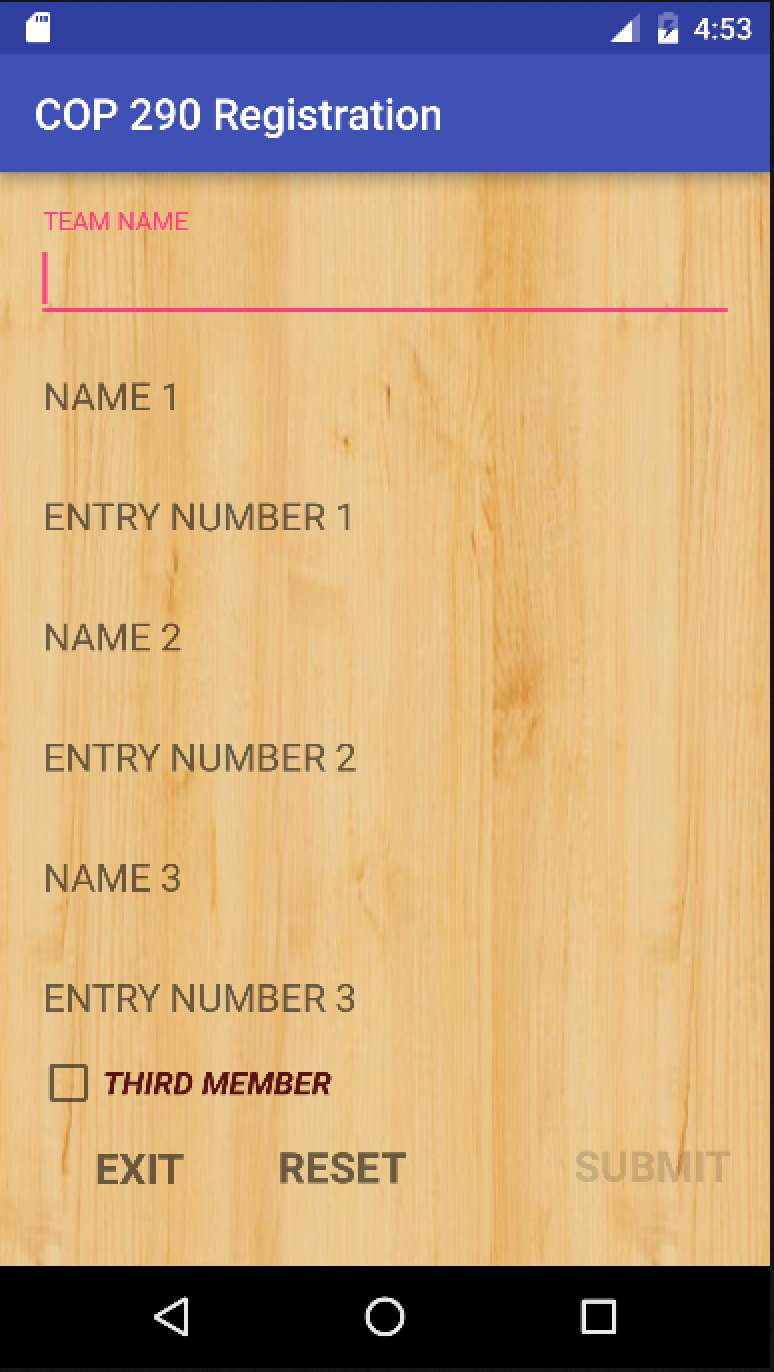
\includegraphics[scale=.7]{MAINSCREENFINAL.png}
	        \captionof{figure}{Main Screen}
            \end{minipage}
            \begin{minipage}{\linewidth}
	        \centering
	        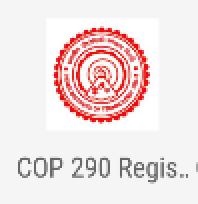
\includegraphics[scale=.5]{LOGO.png}
	        \captionof{figure}{LOGO}
            \end{minipage}
            \\



\begin{itemize}
\item On opening the application the Main Screen (Figure 1), will be visible to the User. The screen contains the following fields:-
\begin{enumerate}
\item \textbf{TEAM NAME:} This is the Text Field where the user enters the \textit{TEAM NAME}. 
\item \textbf{NAME 1:} This is the Text Field where the user enters the \textit{NAME OF FIRST MEMBER}. It is disabled initially.
\item \textbf{ENTRY NUMBER 1:} This is the Text Field where the user enters the \textit{ENTRY NUMBER OF FIRST MEMBER}. It is disabled initially.
\item \textbf{NAME 2:} This is the Text Field where the user enters the \textit{NAME OF SECOND MEMBER}. It is disabled initially.
\item \textbf{ENTRY NUMBER 2:} This is the Text Field where the user enters the \textit{ENTRY NUMBER OF SECOND MEMBER}. It is disabled initially.
\item \textbf{NAME 3:} This is the Text Field where the user enters the \textit{NAME OF THIRD MEMBER}. It is disabled initially.
\item \textbf{ENTRY NUMBER 3:} This is the Text Field where the user enters the \textit{ENTRY NUMBER OF THIRD MEMBER}. It is disabled initially.
\item \textbf{CHECK BOX:} This is checked if the User wants to enter third member information. 
\item \textbf{SUBMIT:} On clicking this button the User information is \textit{Submitted}.
\item \textbf{RESET:} On clicking this button the form is reset.
\end{enumerate}
The background has a wooden texture, with a light shade for easy visibility. Since the information of the third member can be entered only if the User checks the \textit{CHECK BOX}, it gives the option to the User to either register \textit{TWO} or \textit{THREE} Users.
\\
Other than the Main Screen Dialog Boxes will appear once the User clicks the \textit{SUBMIT BUTTON} depending on the information submitted by the User which is authenticated.

\item The enable/disable conditions of the text fields and buttons are listed as follows:
\begin{center}

\begin{tabular}{ |p{3cm}||p{5cm}|p{5cm}|  }
 \hline
 \multicolumn{3}{|c|}{ENABLE/DISABLE List} \\
 \hline
FIELD     & ENABLE & DISABLE\\

 \hline
 TEAM NAME & - & -  \\ 
 NAME 1 & entering text in TEAM NAME & initially \\
 ENTRY NO. 1 & entering text in TEAM NAME & initially  \\
 NAME 2 &  entering text in NAME 1 & initially \\
 ENTRY NO. 2 & entering text in NAME 1 & initially  \\
 NAME 3 & checking the CHECK BOX & unchecking the CHECK BOX \\
 ENTRY NO. 3 & checking the CHECK BOX & unchecking the CHECK BOX \\
 CHECK BOX & - & -  \\
 SUBMIT BUTTON & required fields are entered & any text field is empty  \\
 \hline
\end{tabular}
\end{center}
The text fields have been animated in the following ways:
\begin{center}
\begin{tabular}{ |p{4cm}||p{9cm}|  }
 \hline
 \multicolumn{2}{|c|}{ANIMATIONS LIST} \\
 \hline
 FIELD  &ANIMATIONS\\
 \hline
 NAME 1 & on entering text in TEAM NAME it flies in from left  \\
 ENTRY NO. 1 & on entering text in TEAM NAME it flies in from left  \\
 NAME 2 &  on entering text in NAME 1 it flies in from left   \\
 ENTRY NO. 2 & on entering text in NAME 1 it flies in from left  \\
 NAME 3 & on checking the CHECK BOX it flies in from left \\
 ENTRY NO. 3 & checking the CHECK BOX  \\

 \hline
\end{tabular}
 \end{center}

\item In addition to at each a toast is raised indicating the User what he is doing and he is supposed to do next.

\begin{figure}[h!]
	\centering
	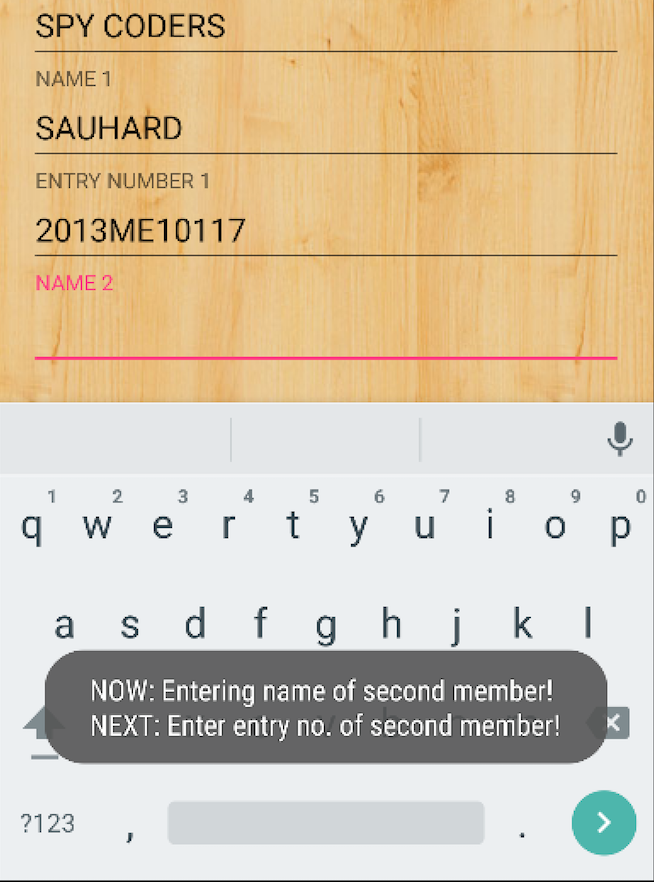
\includegraphics[scale=.5]{toast.png}
	\caption{TOAST}
\end{figure}



\item The screen has three click-able fields i.e. \textit{CHECK BOX, EDIT BUTTON} and \textit{SUBMIT BUTTON}. The actions are listed below:
\begin{enumerate}
\item \textit{\textbf{SUBMIT BUTTON:}} It performs the dual function of sending the information to the server and authenticating it before sending it. Hence on clicking the \textit{SUBMIT BUTTON} a dialog box will appear indicating the action undertaken. The various Dialog boxes and there conditions are listed below:        

\item \textbf{\textit{CHECK BOX:}} This when checked enables the user to enter the information for Third Member by enabling the Text Fields.
\item \textit{\textbf{RESET BUTTON:}} This enables the User to Reset the entire form.

\end{enumerate}


\end{itemize}

\section{Implementation Details}

\begin{itemize}
\item 
Functions were used to eliminate repeatitive statements.
We used an inbuilt data structure LinkedHashMap. This is a  constructor that creates a linked hash map which iterates in the order in which its entries were last accessed, from least-recently accessed to most-recently (access-order). 
\item The error is handled in two stages: 
\begin{enumerate}
\item \textbf{WHILE ENTERING:} This feature checks the Format of the Name and Entry Number and raise an error in case its incorrect.
\\
            \\
            \begin{minipage}{\linewidth}
	        \centering
	        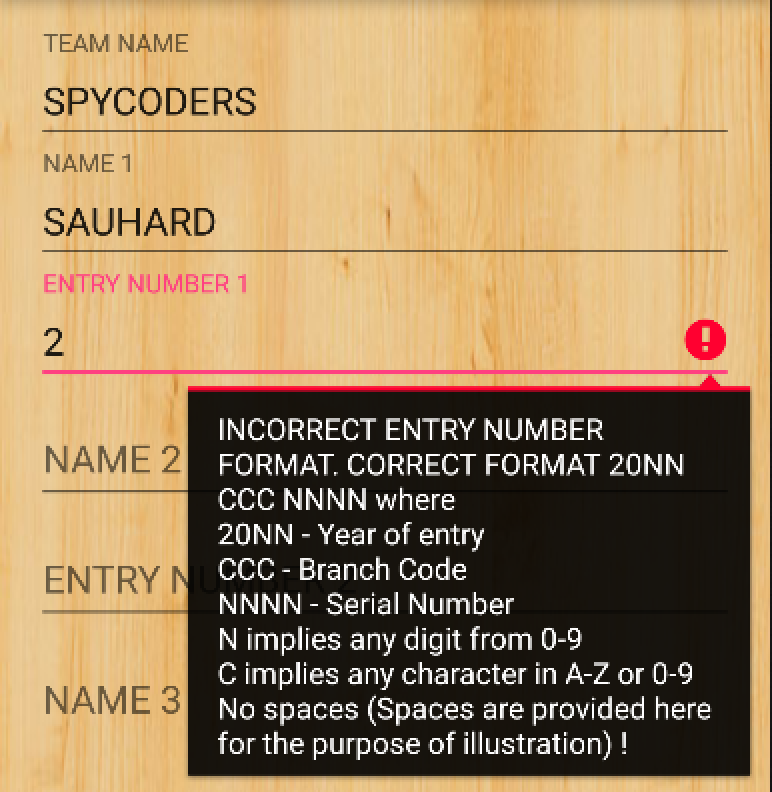
\includegraphics[scale=.7]{WRONG_ENTRY_NUM.png}
	        \captionof{figure}{WRONG ENTRY NUMBER-1}
            \end{minipage}
            \\
            \\
            \\
            \begin{minipage}{\linewidth}
	        \centering
	        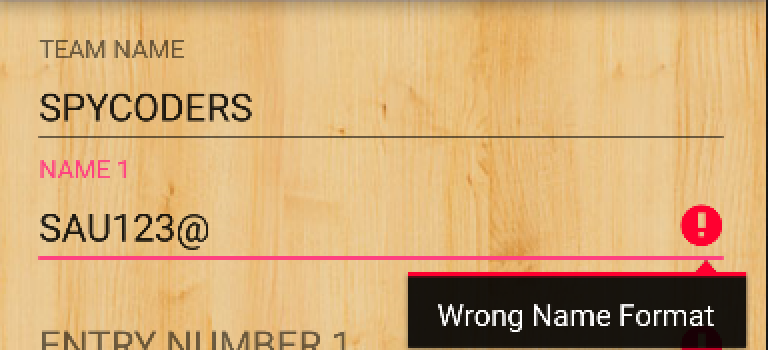
\includegraphics[scale=.7]{WRONG_NAME.png}
	
	        \captionof{figure}{WRONG NAME}
            \end{minipage}
            \\
            \\
\item \textbf{SUBMIT BUTTON}
\begin{enumerate}
            \item \textit{INCORRECT ENTRY NUMBER FORMAT:} It indicates the User has entered a Entry Number in wrong format. The button \textbf{OK} is present, which can be pressed to go back to the form with focus to the text field with the error.
            \\
            \\
            \begin{minipage}{\linewidth}
	        \centering
	        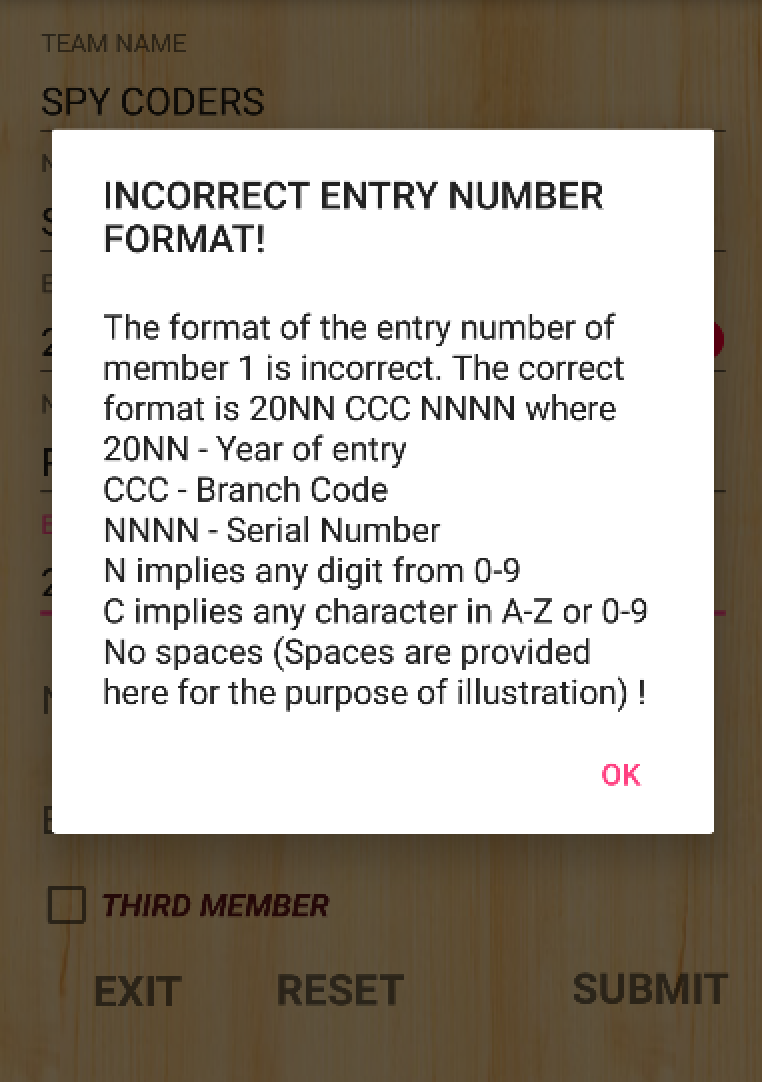
\includegraphics[scale=.5]{INCORRECT_NUMBER_FORMAT}
	        \captionof{figure}{WRONG ENTRY NUMBER-2}
            \end{minipage}
            
            \item \textit{ENTRY NUMBER REPEAT:} It indicates the User has entered an Entry Number that is already registered.The button \textbf{OK} is present, which can be pressed to go back to the form with focus to the text field with the error.\\
            \\
            \\
            \\
            \\
            \par
             \begin{minipage}{\linewidth}
        	    \centering
        	    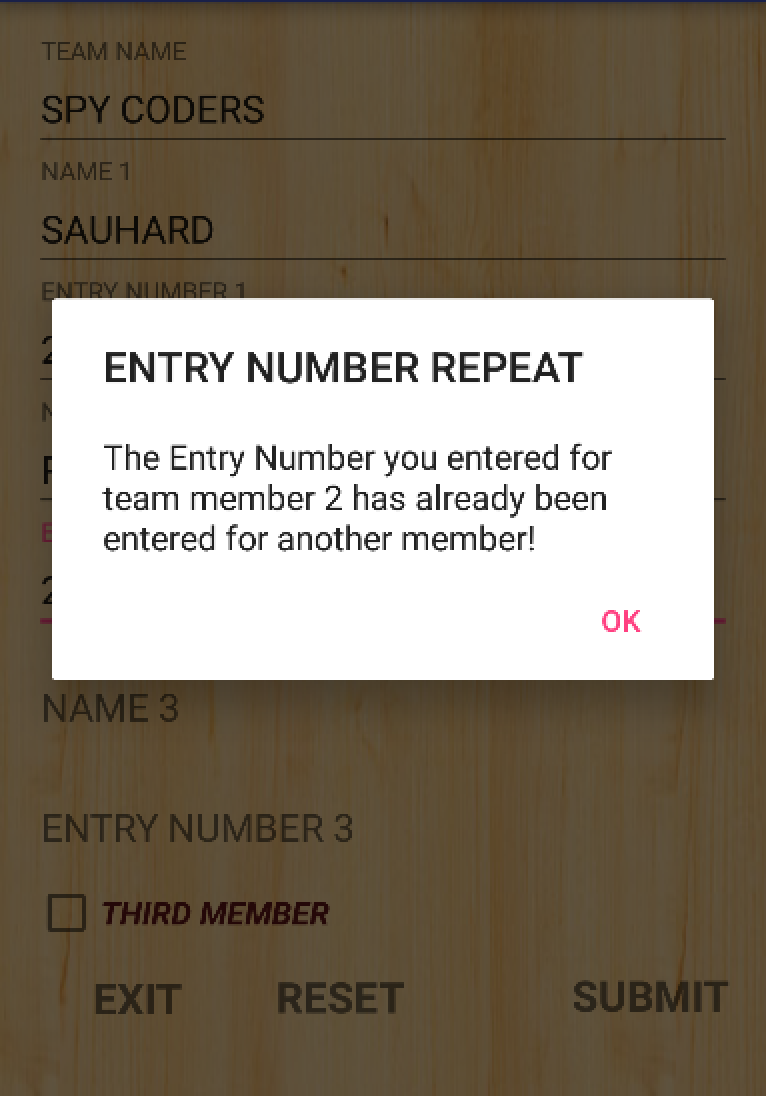
\includegraphics[scale=.7]{ENTRY_NUMBER_REPEAT.png}
        	    \captionof{figure}{ENTRY NUMBER REPEAT}
            \end{minipage}
            \\
            \\
            
            \item \textit{TEAM MEMBER'S NAME ENTRY NUMBER MISMATCH:} It indicates the User has entered a Name and Entry Number that do not match.The button \textbf{OK} is present, which can be pressed to go back to the form with focus to the text field with the error.
            \\
            \\
            \par
             \begin{minipage}{\linewidth}
        	    \centering
	            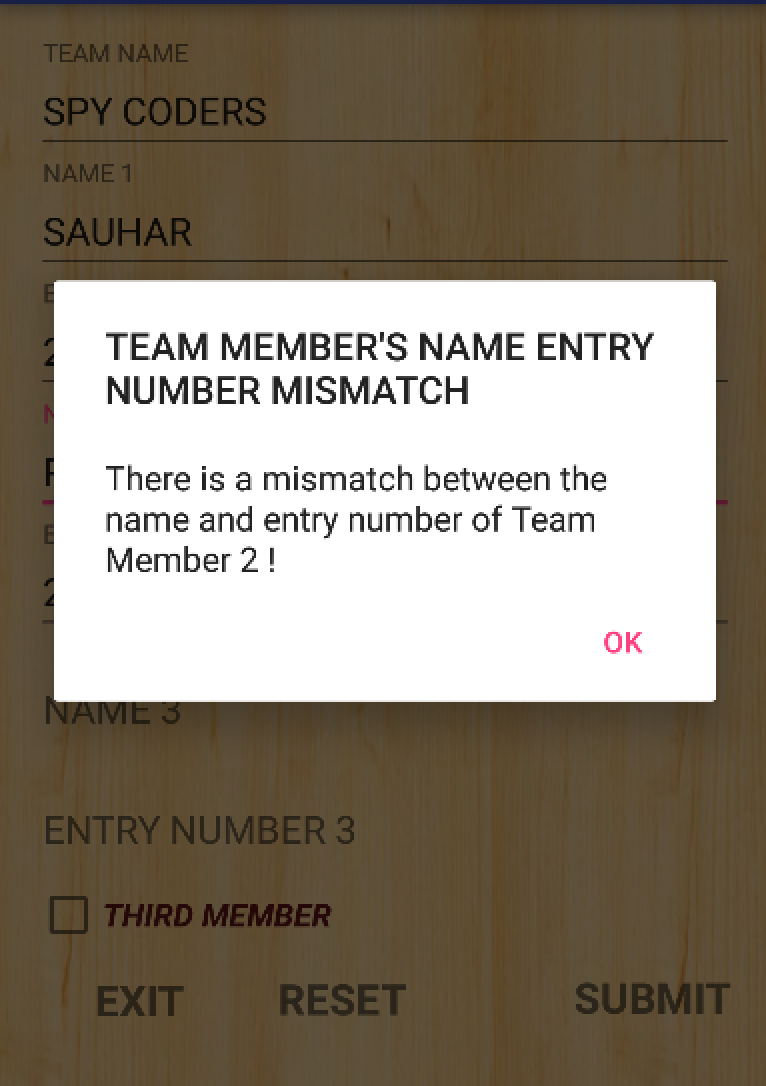
\includegraphics[scale=.7]{TEAM_MEMBER'S_NAME_ENTRY_NUMBER_MISMATCH.png}
	    	    \captionof{figure}{TEAM MEMBER'S NAME ENTRY NUMBER MISMATCH}
            \end{minipage}
            \\
            \\
            \item \textit{TEAM MEMBER NOT REGISTERED FOR COP290 COURSE:} It indicates the User has entered a Name and Entry Number that are not registered for the course.The button \textbf{OK} is present, which can be pressed to go back to the form with focus to the text field with the error.
            \\
            \\
            \begin{minipage}{\linewidth}
	        \centering
	        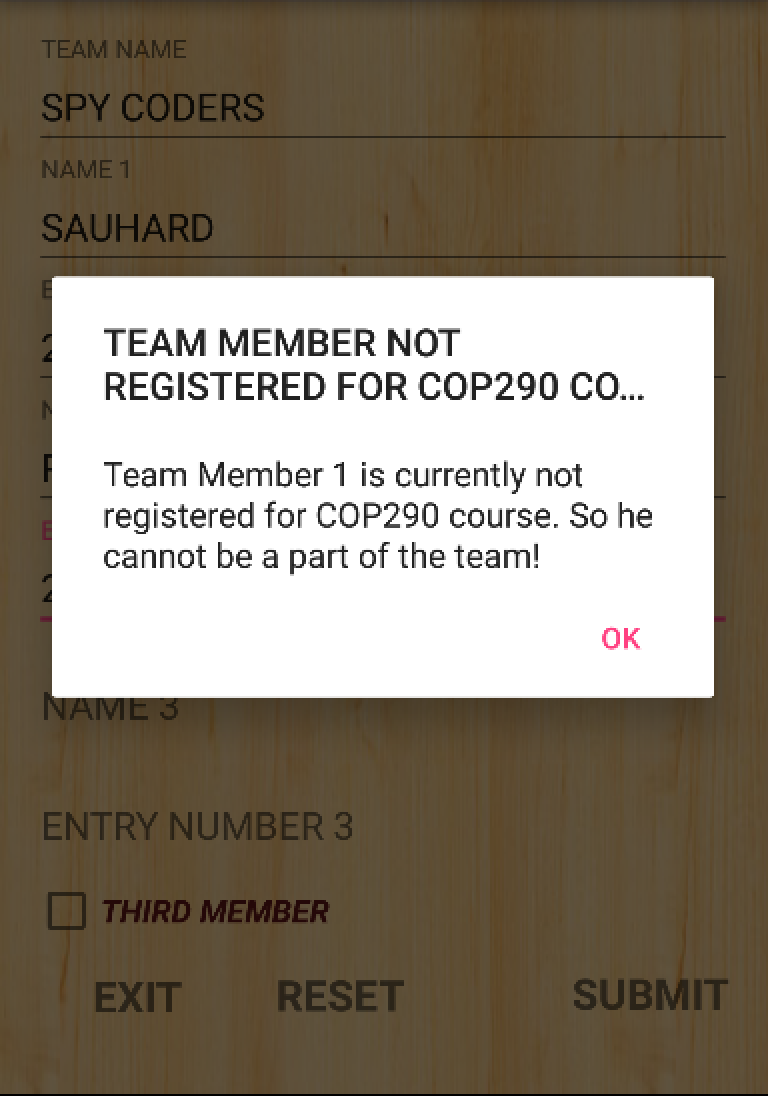
\includegraphics[scale=.7]{TEAM_MEMBER_REGISTERED_FOR_COP.png}
	        \captionof{figure}{TEAM MEMBER REGISTERED FOR COP}
            \end{minipage}
            \\
            \\
            \\
            \\
            
            
            
            \item \textit{CONNECTION ERROR:} It indicates the device is not connected to the network. The button \textbf{RETRY} enables the User to try to submit the form again, the button \textbf{BACK} enables the User to back to the form again and the button \textbf{EXIT} enables the User to exit from the form.
            \\
            \\
            \begin{minipage}{\linewidth}
	        \centering
	        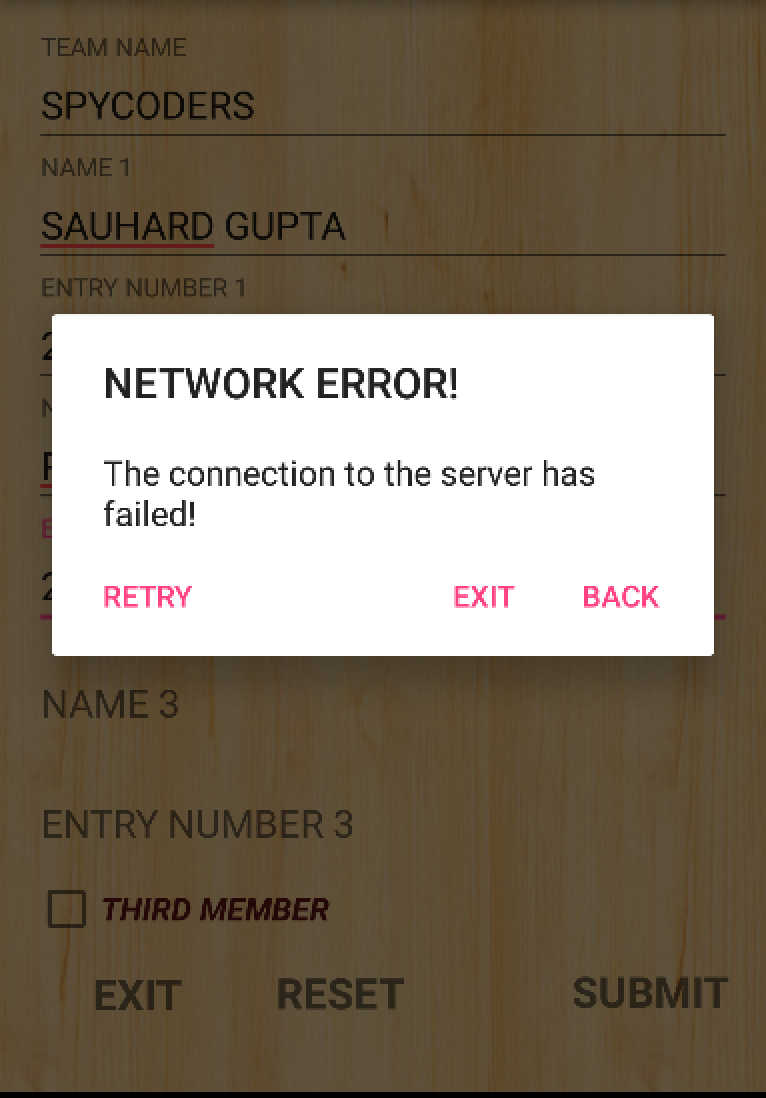
\includegraphics[scale=.7]{CONNECTION_FAILED.png}
	        \captionof{figure}{CONNECTION FAILED}
            \end{minipage}
            \\
            \\
            \\
            \\
            
            \item \textit{REGISTERED USER:} It indicates the User has entered a Entry Number that is already registered. The button \textbf{EDIT} enables the User to go back to the form again and edit it and the button \textbf{EXIT} enables the User to exit from the form.
            \\
            \\
            \begin{minipage}{\linewidth}
	        \centering
	        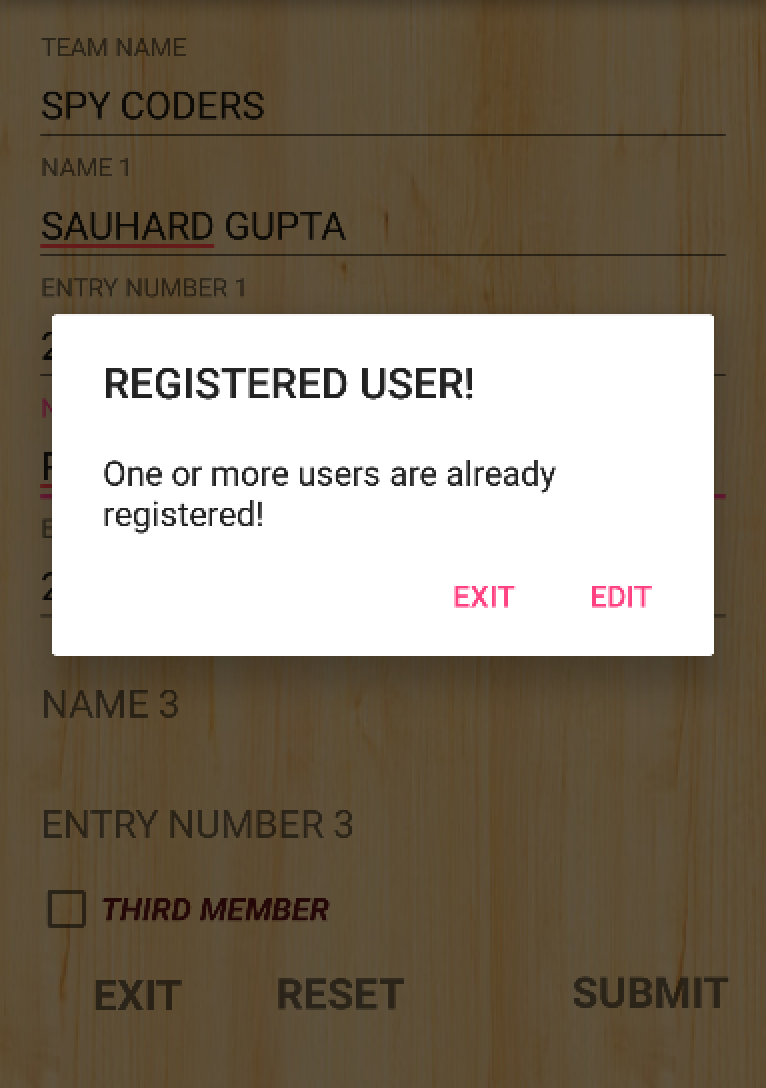
\includegraphics[scale=.7]{REGISTERED_USER.png}
	        \captionof{figure}{ALREADY REGISTERED USER}
            \end{minipage}
            \\
            \\

        \end{enumerate}
        \end{enumerate}
        
	
\item  
To send the User information to the server we first added the following libraries:
\begin{enumerate}
    \item \textbf{java.net.URL :} to set the URL. 
    \item \textbf{java.net.HttpURLConnection :} to connect, post and receive.

\item \textbf{java.net.URLEncoder}
\end{enumerate}
Next to post this information we used the \textbf{"POST"} method of \textit{HttpURLConnection}.
\item All the Strings used in the app which will potentially get displayed to the User during run-time, are managed in a separate file /res/file/strings.xml. This helps in better management of the strings and provides scope for translation of app into various languages.



























\end{itemize}

Report made and compiled by {\em Sauhard Gupta 2013ME10117}.

\bibliography{references}\\
\textbf{\textit{REFERENCES:-}}\\
\\
http://developer.android.com \\
http://stackoverflow.com    \\
https://github.com          \\
https://slack.com   (https://spycoderscop290.slack.com)         \\
For adding animation:- https://www.youtube.com/watch?v=0gElZRDtWHs  \\
http://stackoverflow.com/questions/15564614/how-to-restart-an-android-application-programmatically\\
http://ldap1.iitd.ernet.in/LDAP/courses/COP290.shtml \\
http://agni.iitd.ernet.in/cop290/assign0/register/ \\
https://docs.oracle.com/javase/tutorial/networking/urls/readingWriting.html \\
http://stackoverflow.com/questions/10500775/parse-json-from-httpurlconnection-object \\
http://developer.android.com/guide/topics/ui/dialogs.html\\
http://stackoverflow.com/questions/15564614/how-to-restart-an-android-application-programmatically\\
http://stackoverflow.com/questions/8258725/strict-mode-in-android-2-2\\
http://www.donnfelker.com/android-validation-with-edittext/\\
https://www.sharelatex.com/learn\\
https://docs.oracle.com/javase/7/docs/api/java/util/LinkedHashMap.html\\
http://www.designbolts.com/wp-content/uploads/2013/02/Free-Seamless-Wood-Textures-Patterns-For-3D-Mapping-2.jpg\\
http://btis.iitd.ac.in/IITD-logo.gif\\


\end{document}